\documentclass[11pt]{article} 
\usepackage[english]{babel}
\usepackage[utf8]{inputenc}
\usepackage[margin=0.5in]{geometry}
\usepackage{amsmath}
\usepackage{amsthm}
\usepackage{amsfonts}
\usepackage{amssymb}
\usepackage[usenames,dvipsnames]{xcolor}
\usepackage{graphicx}
\usepackage[colorinlistoftodos, color=orange!50]{todonotes}
\usepackage{hyperref}
\usepackage[numbers, square]{natbib}
\usepackage{fancybox}
\usepackage{epsfig}
\usepackage{soul}
\usepackage[framemethod=tikz]{mdframed}
\usepackage[shortlabels]{enumitem}
\usepackage[version=4]{mhchem}
\usepackage{multicol}
\usepackage{forest}
\usepackage{mathtools}
\usepackage{comment}
\usepackage{enumitem}
\usepackage[utf8]{inputenc}
\usepackage{listings}
\usepackage{color}
\usepackage[numbers]{natbib}
\usepackage{subfiles}
\usepackage{algorithm}
\usepackage[noend]{algpseudocode}


\DeclarePairedDelimiter\ceil{\lceil}{\rceil}
\DeclarePairedDelimiter\floor{\lfloor}{\rfloor}

\newtheorem{prop}{Proposition}[section]
\newtheorem{thm}{Theorem}[section]
\newtheorem{lemma}{Lemma}[section]
\newtheorem{cor}{Corollary}[prop]

\theoremstyle{definition}
\newtheorem{definition}{Definition}

\theoremstyle{definition}
\newtheorem{required}{Problem}
\newtheorem*{requiredHC}{Problem HC}

\theoremstyle{definition}
\newtheorem{ex}{Example}

\newcommand{\interval}[4]{\draw (#2, #1) -- (#3, #1); % Usage: \interval{height}{start}{end}{label}
\draw (#2, #1-0.11) -- (#2, #1+0.11); % draw left whisker
\draw (#3, #1-0.11) -- (#3, #1+0.11); % draw right whisker
\node[] at (#2-0.25, #1) {#4};
}


\setlength{\marginparwidth}{3.4cm}
%#########################################################

%To use symbols for footnotes
\renewcommand*{\thefootnote}{\fnsymbol{footnote}}
%To change footnotes back to numbers uncomment the following line
%\renewcommand*{\thefootnote}{\arabic{footnote}}

% Enable this command to adjust line spacing for inline math equations.
% \everymath{\displaystyle}

% _______ _____ _______ _      ______ 
%|__   __|_   _|__   __| |    |  ____|
%   | |    | |    | |  | |    | |__   
%   | |    | |    | |  | |    |  __|  
%   | |   _| |_   | |  | |____| |____ 
%   |_|  |_____|  |_|  |______|______|
%%%%%%%%%%%%%%%%%%%%%%%%%%%%%%%%%%%%%%%

\title{
\normalfont \normalsize 
\textsc{CSCI 3104 Spring 2022 \\ 
Instructor: Profs. Chen and Layer} \\
[10pt] 
\rule{\linewidth}{0.5pt} \\[6pt] 
\huge Problem Set 5 \\
\rule{\linewidth}{2pt}  \\[10pt]
}
%\author{Your Name}
\date{}

\begin{document}
\definecolor {processblue}{cmyk}{0.96,0,0,0}
\maketitle


%%%%%%%%%%%%%%%%%%%%%%%%%
%%%%%%%%%%%%%%%%%%%%%%%%%%
%%%%%%%%%%FILL IN YOUR NAME%%%%%%%
%%%%%%%%%%AND STUDENT ID%%%%%%%%
%%%%%%%%%%%%%%%%%%%%%%%%%%
\noindent
Due Date \dotfill March 1 \\
Name \dotfill \textbf{Chengming Li} \\
Student ID \dotfill \textbf{109251991} \\
Collaborators \dotfill \textbf{N/A}

\tableofcontents

\section*{Instructions}
\addcontentsline{toc}{section}{Instructions}
 \begin{itemize}
	\item The solutions \textbf{must be typed}, using proper mathematical notation. We cannot accept hand-written solutions. Useful links and references on \LaTeX can be found \href{https://canvas.colorado.edu/courses/75824/pages/latex}{here on Canvas}.
	\item You should submit your work through the \textbf{class Canvas page} only. Please submit one PDF file, compiled using this \LaTeX \ template.
	\item You may not need a full page for your solutions; pagebreaks are there to help Gradescope automatically find where each problem is. Even if you do not attempt every problem, please submit this document with no fewer pages than the blank template (or Gradescope has issues with it).

	\item You are welcome and encouraged to collaborate with your classmates, as well as consult outside resources. You must \textbf{cite your sources in this document.} \textbf{Copying from any source is an Honor Code violation. Furthermore, all submissions must be in your own words and reflect your understanding of the material.} If there is any confusion about this policy, it is your responsibility to clarify before the due date. 

	\item Posting to \textbf{any} service including, but not limited to Chegg, Reddit, StackExchange, etc., for help on an assignment is a violation of the Honor Code.

\end{itemize}


\newpage
\section{Standard 14 - Analyzing Code III: (Writing down recurrences)}

\begin{required} \label{Recursive1}
Write down the recurrence relation for the runtime complexity of these algorithms. \textbf{Don't forget to include the base cases.}

\subsection{Problem 1(a)}

\begin{algorithm}
\caption{Writing Recurrences 1}\label{alg:Recurrence1}
\begin{algorithmic}[1]
\Procedure{Foo}{$\text{Integer } n$}
\If{$n \leq 3$} 
\Return
\EndIf

\noindent \\
\State $\text{Foo}(n/3)$
\State $\text{Foo}(n/3)$
\State $\text{Foo}(n/3)$ \\

\For{$i \gets 1; i \leq 2*n; i \gets i+1 $}
	\State \textbf{print} \text{``Hi, Hi"}
\EndFor
\EndProcedure
\end{algorithmic}
\end{algorithm}

\begin{proof}[Answer]
%Your answer here
\end{proof}


%We have included a LaTeX code sample that may be helpful for displaying recurrences
\begin{comment}
\begin{align*}
T(n) &= \begin{cases}
5 & : \text{if } n \geq 0, \\
7 & : \text{if } n < 0.
\end{cases}
\end{align*}
\end{comment}




\newpage


\subsection{Problem 1(b)}

\begin{algorithm}
\caption{Writing Recurrences 2}\label{alg:Recurrence2}
\begin{algorithmic}[1]
\Procedure{Foo}{$\text{Integer } n$}
\If{$n \leq 4$}
\Return
\EndIf

\noindent \\
\State $\text{Foo}(n/4)$
\State $\text{Foo}(n/4)$
\State $\text{Foo}(n/3)$ \\

\For{$i \gets 1; i \leq n; i \gets i*2 $}
	\State \textbf{print} \text{``Hi, Hi"}
\EndFor
\EndProcedure
\end{algorithmic}
\end{algorithm}
\end{required}

\begin{proof}[Answer]
%Your answer here
\end{proof}

\newpage

\section{Standard 15 - Unrolling}

\begin{required} \label{Unrolling1}
Consider the following recurrences and solve them using the unrolling method (i.e. find a suitable function $f(n)$ such that $T(n) \in \Theta(f(n))$). 
\begin{enumerate} [label=(\alph*)]
    \item 
\begin{align*}
T(n) = \begin{cases}
2 & : n < 3, \\
2T(n - 3) + 2 & : n \geq 3.
\end{cases}
\end{align*}

\begin{proof}[Answer]

\textbf{Assuming we need unrolling k times\\}
Then:\\
\begin{align*}
n-3k &< 3 \\
k &>  \frac {3-n}{-3}\\
k &> \ceil{\frac{n-3}{3}}\\
k &\approx \frac{n-3}{3}
\end{align*}

\textbf{Then, write down some iterations\\}
\begin{align*}
T(n) &= 2T(n-3)+2\\
&= 2 + 2 (2T(n-6) + 2)\\
&= 2^{2} T(n-3*2)+2^2 + 2\\
&= 2 + 2[2(2T(n-9)+2)+ 2]\\
&= 2^3 T(n-3*3) + 2^3 + 2^2 + 2\\
&= 2^{k}T(n-3k) + 2^{k}2 + 2^{k-1}2 +... + 2^{0}2
\end{align*}

\textbf{Thus, the recurrence is :\\ }
\begin{align*}
T(n) &= 2 * 2^{\frac{n-3}{3}} + \sum_{i=0}^{\frac{n-3}{3}} 2^i\\
&=  2 * 2^{\frac{n-3}{3}} + 2* \frac {2^{\frac{n-3}{3} + 1} -1 }{2-1}\\
&= 2 * 2^{\frac{n-3}{3}} + 2*2*2^{\frac{n-3}{3} + 1}- 2\\
&= 2^{\frac{n-3}{3}} (2+4) -2
\end{align*}
\textbf{Higher order term dominates whole expression. So, $T(n)$ $\in \Theta(6*2^{\frac{n-3}{3}}) = \Theta(2^{\frac{n}{3}})$} 
%Your answer here
\end{proof}

\newpage
\item
\begin{align*}
T(n) = \begin{cases}
3 & : n < 2, \\
T(n-2) + 4n & : n \geq 2.
\end{cases}
\end{align*}

\begin{proof}[Answer]
\textbf{Assuming we need unrolling k times\\}
Then:\\
\begin{align*}
n-2k &< 2 \\
k &>  \frac {2-n}{-2}\\
k &> \ceil{\frac{n-2}{2}}\\
k &\approx \frac{n-2}{2}
\end{align*}

\textbf{Then, write down some iterations\\}
\begin{align*}
T(n) &= T(n-2)+4n\\
&= T(n-2*2) + 4(n-2) + 4n\\
&= T(n-2*3) + 4(n-2*2) + 4(n-2) + 4n\\
&= T(n-2k) + 4(n-2k) + ... + 4n
\end{align*}

\textbf{Thus, the recurrence is :\\ }
\begin{align*}
T(n) &= 3 * 2^{\frac{n-2}{2}} +4 *  \sum_{i=0}^{\frac{n-2}{2}} (n-2i)\\
&=  3 * 2^{\frac{n-2}{2}} + 4n * \sum_{i=0}^{\frac{n-2}{2}} 1 +8\sum_{i=0}^{\frac{n-2}{2}} i\\
&=  3 * 2^{\frac{n-2}{2}} + 4n(\frac{n-2}{2} + 1) -8 \frac{(n-2)/2 * ((n-2)/2 + 1)}{2} \\
&=  3 * 2^{\frac{n-2}{2}} + 4n(\frac{n-2}{2} + 1) - (n^2 - 2n)\\
&\approx  3*\Theta(2^{(n-2)/2}) + 4\Theta(n^2) - \Theta(n^2) 
\end{align*}
\textbf{Higher order term dominates whole expression. So, $T(n)$ $\in \Theta(3*2^{\frac{n-2}{2}}) = \Theta(2^{\frac{n}{2}})$} 
%Your answer here
\end{proof}
\end{enumerate}

\end{required}

\newpage
\section{Standard 16 - Tree Method.}

\begin{required}
Consider the recurrence $T(n)$ below. Using the {\bf tree method}, determine a suitable function $f(n)$ such that $T(n) \in \Theta(f(n))$. Clearly show all steps. Note the following:
\begin{itemize}
\item You may assume, without loss of generality, that $n$ is a power of $3$ (i.e., $n = 3^{k}$ for some integer $k \geq 0$).
\item You may hand-draw your tree and embed it, provided it is legible and we do not have to rotate our screens to read it. However, \textbf{all your calculations must be typed}.
\end{itemize}

\[
T(n) = \begin{cases} 2, &  n < 3 \\ 
2T(n/3) + n^{2}, &  \text{otherwise.} \end{cases}
\]

\end{required}

\begin{proof}[Answer]
\textbf{Finding the depth of tree first}
\begin{align*}
\frac{n}{3^k} &< 3\\
\frac{n}{3} &< 3^k\\
\ln{n/3} &k\ln{3}\\
k &> log_3(\frac{n}{3})\\
k &\approx log_3(\frac{n}{3})
\end{align*}

\textbf{Tree Method:}
\begin{center}
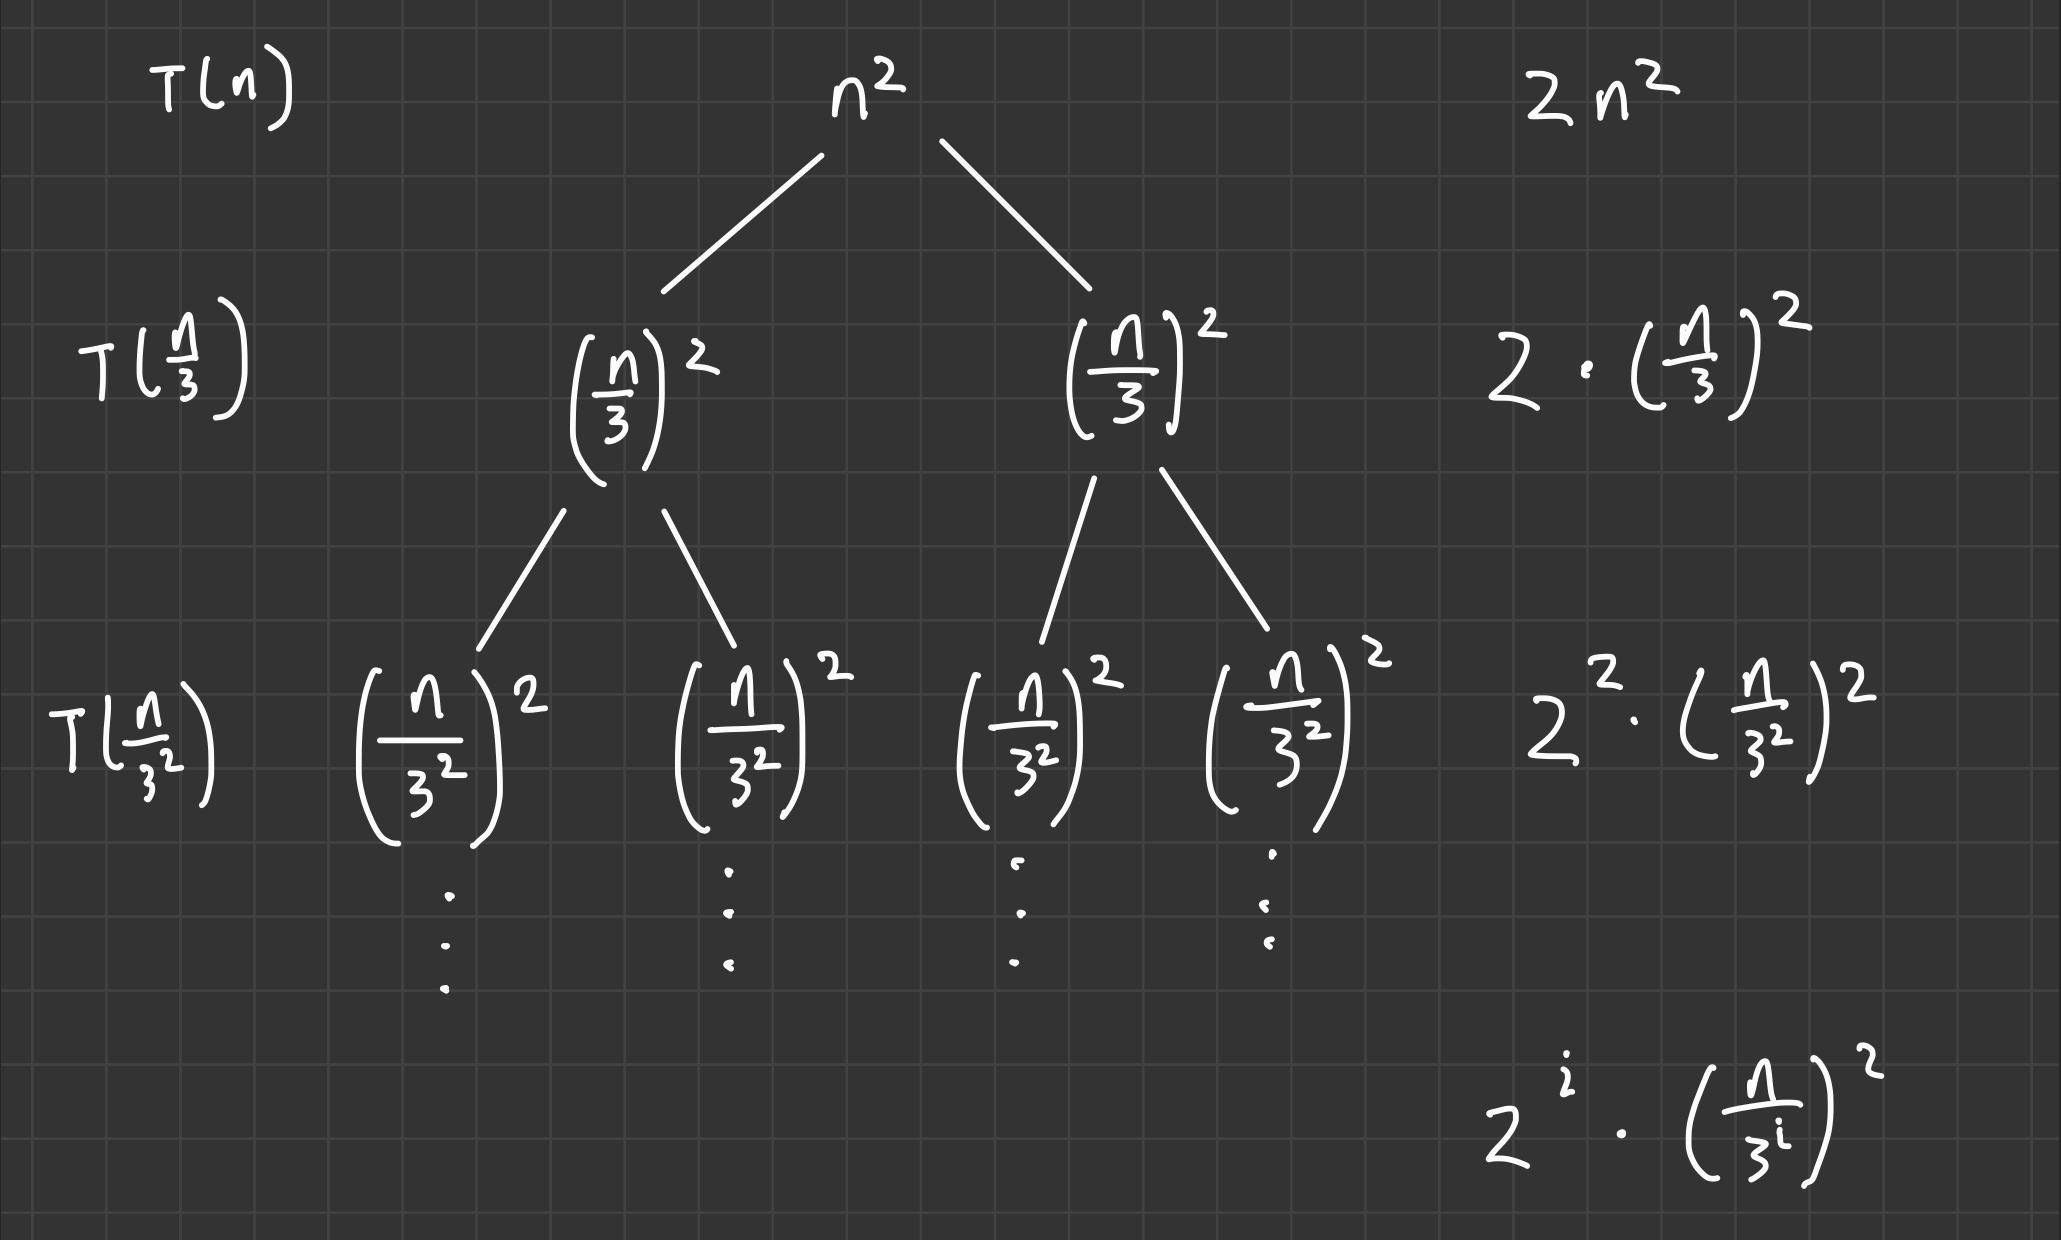
\includegraphics[width=0.7\textwidth]{HW5P3.PNG}
\end{center}

\textbf{Finding running time:\\}
\begin{align*}
T(n) &= \sum _{i=0}^{log_3\frac{n}{3}}2^i\cdot \left(\frac{n}{3^i}\right)^2\\
&= n^2\sum _{i=0}^{log_3\frac{n}{3}}2^i\cdot \left(\frac{1}{3^i}\right)^2\\
&= n^2\sum _{i=0}^{log_3\frac{n}{3}}\left(\frac{2}{9}\right)^i
\end{align*}
% YOUR ANSWER HERE
\end{proof}


\end{document} % NOTHING AFTER THIS LINE IS PART OF THE DOCUMENT